\chapter*{Week 4: Loops}
\addcontentsline{toc}{chapter}{Week 4: Loops}
\setcounter{chapter}{4}
\setcounter{section}{0}

\begin{abstract}
This week will cover:
\begin{enumerate}
    \item Learn about loops in C++:
    \begin{itemize}
        \item While loops
        \item Do-while loops
        \item For loops
    \end{itemize}
    \item Learn to convert between loop formats
    \item Learn to debug your loops
    \item Arrays
\end{enumerate}
    
\end{abstract}

\section{Background}
Loops are a tool that allows us to repeat a block of code. The number of repetitions is controlled by the conditions of the loop, and can range anywhere from never executing, executing a fixed number of times, or executing an infinite number of times. Loops will execute for as long as their condition is satisfied; once the condition is not true, the loop will stop and the program will continue. The structure of these conditions can vary depending on the type of loop used. There are three main types of loop we use in C++; the while loop, the do-while loop, and the for loop.

\subsection{While Loops}
While loops are the most basic form of loops. Their structure looks like:

\begin{minted}{c++}
while (condition)
{
    //code to execute
}
\end{minted}

Here, $while$ is a C++ reserved word, $condition$ should be a Boolean expression that will evaluate to either \textbf{true} or \textbf{false}, and the comment between the brackets is where we would add code to execute. If the condition is true, then the specified statement(s) within the loop are executed. After running once, the Boolean expression is re-evaluated. If the condition is true, the specified statement(s) are executed again. This process of evaluation and execution is repeated until the condition becomes \textbf{false}.

\begin{example}
Here is an example of a while loop where the condition is based on user input. 
\begin{minted}{c++}
int userChoice = 1;
while (userChoice != 0)
{
   cout << "Do you want to see the question again?" << endl; 
   cout << "Press 0 if no, any other number if yes." << endl;
   cin >> userChoice;
}
\end{minted}
Entering 0 will terminate the loop, but any other number will cause the loop to execute again. Note how we must initialize the condition before the loop starts. Setting userChoice = 1 ensures that the while loop will run at least once.
\end{example}

\begin{example}
    Here is an example of a while loop where the condition is based on a counter.
    \begin{minted}{c++}
int i = 0; 
while (i < 5)
{
	cout << i << endl;
	i = i + 2;
}
    \end{minted}
    Notice how you must manually initialize i=0 and then manually increment i by 2.
\end{example}

\subsection{Do-While Loops}
The do-while loop is a variant of the while loop. The critical difference with a do-while loop is that the block of code we wish to execute is written before the condition. The structure of a do-while loop looks like this:
\begin{minted}{c++}
do {
  // code block to be executed
}
while (condition);
\end{minted}

In a do-while loop, the block of code is executed once before the condition is checked. This means we will never entirely skip a do-while loop. You will often find this type of loop to be useful when gathering user input, like the example shown below.

\begin{example}
    Here is an example of the while loop from example 1.1.1. rewritten as a do-while loop.

    \begin{minted}{c++}
int userChoice;
do {
   cout << "Do you want to see the question again?" << endl; 
   cout << "Press 0 if no, any other number if yes." << endl;
   cin >> userChoice;
}  
while (userChoice != 0);
    \end{minted}

    Note that here we do not have to initialize user choice before the loop begins.
    
\end{example}


\subsection{For Loops}
You will frequently come across instances where you already know the number of iterations you would like your loop to complete, like example 1.1.2 shown above. In these cases, there is a special loop that has a counter built in rather than needing to keep track on your own. For loops have three elements:
\begin{itemize}
    \item Initialization: It must initialize a counter variable to a starting value. Note: When initializing your counter, you can choose to either declare a new variable or use an existing variable. If you declare a new variable in your initialization, it will only exist in the \textbf{scope} of the loop; this means once the loop concludes, you cannot access that variable again. 
    \item Condition: If it is true, then the body of the loop is executed. If it is false, the body of the loop does not execute and jumps to the next statement(s) just after the loop.
    \item Update: Updates the counter variable during each iteration
\end{itemize}

The basic structure of a for loop looks like this:

\begin{minted}{c++}
for (initialization; condition; update)
{
    //code to execute
}
\end{minted}

Here, $for$ is a C++ reserved word. 

\begin{example}
    Here is a section of code that will simply print the word "hello" five times:
    \begin{minted}{c++}
for (int count = 0; count < 5; count++)
{
	cout << "hello" << endl;
}
    \end{minted}
    Notice the following three parts of the for loop:

    \begin{itemize}
        \item count is initialized to 0,
        \item the conditional expression is count < 5
        \item count++ to increment the count value by one
    \end{itemize}

\end{example}

\begin{example}
    Here is an example that would work equivalently to example 1.1.2.:
    \begin{minted}{c++}
for (int i = 0; i < 5; i = i + 2)
{
	cout << i << endl;
}
    \end{minted}
\end{example}

\subsection{Common Errors and Debugging Loops}

Unique errors with loops include:

\begin{itemize}
\item errors with the loop syntax itself, such as your condition or the set of statements in your for loops. Check that you have semicolons and have declared all your variables that you use in this area. 
\item infinite loops, which will frequently present as either a program that never stops running or an error saying something along the lines of memory exceeded or time exceeded. Check your conditions, and make sure the variables that control your condition are updating correctly. 
\item incorrect numbers of iterations, which means you may not be updating your counter correctly or your logic may be incorrect. 
\end{itemize}
Here is a flowchart for helping you figure out (and resolve) what is wrong with your loops:

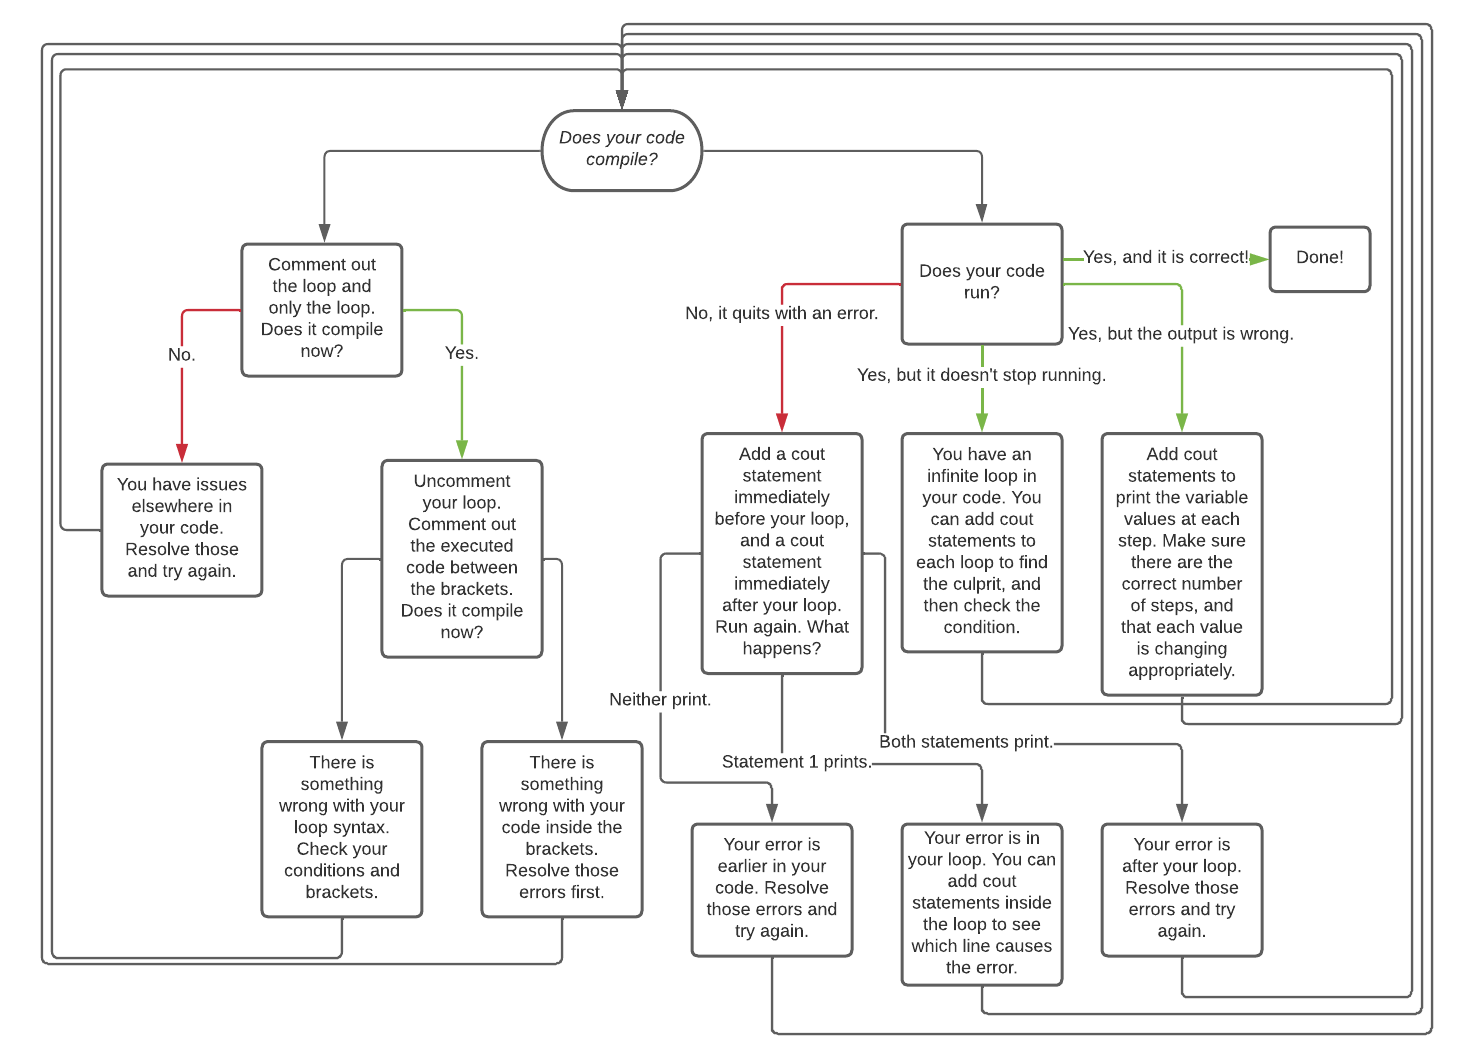
\includegraphics[width=\textwidth]{images/Loop Debugging.png}

Any errors that you may come across either within the bracketed section of your loop or outside of your loop are subject to the same rules as any code we have previously worked with. If you are struggling with errors in those areas, revisit debugging tips from the relevant sections to help you. 

\subsection{Arrays}
An array is a data structure which can store other data types like double, int, char, and boolean, and string. Arrays have both a type and a size.

\subsubsection{Making and Using Arrays}

\textbf{How to declare arrays}
\begin{minted}{c++}
// data_type array_name[declared_size];
bool myBooleans[10];
string myStrings[15];
int myInts[7];
\end{minted}

\textbf{How to initialize arrays (method 1)}
\begin{minted}{c++}
bool myBooleans[4] = {true, false, true, true};
\end{minted}

If you do not declare the size inside the square brackets, the array size will be set to however many entries you provide on the right.

\begin{minted}{c++}
bool myBooleans[] = {true, false, true}; // size = 3
\end{minted}

Note: the size specified in the brackets needs to match the number of elements you wrote in the curly brackets.

\begin{example}
    When the specified size is larger than the actual number of elements, the elements provided in the curly brackets will be the first several elements in the array, while the additional elements will be filled with default values. If it’s an integer/double array, the default values are zero, while if it’s a string array, the default values are empty strings.
    \begin{minted}{c++}
#include <iostream>
using namespace std;
int main()
{
    int intArray[5] = {1,2,3};
    for (int i = 0; i < 5; i ++)
    {
        cout << intArray[i] << " ";
    }
}
    \end{minted}

    Output:

    \mintinline{c++}{1 2 3 0 0}
\end{example}

\begin{example}
    When the specified size is smaller than the actual number of elements, there will be a compilation error.

    \begin{minted}{c++}
#include <iostream>
using namespace std;
int main()
{
    int intArray[3] = {1,2,3,4,5};
}
    \end{minted}

    Output:

    \begin{minted}{c++}
error: excess elements in array initializer
int intArray[3] = {1,2,3,4,5};
                         ^
1 error generated.
    \end{minted}
\end{example}

\textbf{How to Initialize Arrays (Method 2)} You can also initialize elements one by one using a for loop:

\begin{minted}{c++}
int myInts[10];
for (int i = 0; i < 10; i++)
{
    myInts[i] = i;
}
//{0, 1, 2, 3, 4, 5, 6, 7, 8, 9}
\end{minted}

\textbf{How to Access Elements in an Array} We have essentially already had practice with accessing elements in an array, as in C++, string is basically an array of characters. You can access elements in arrays using the same syntax you used for strings:

\begin{minted}{c++}
string greetings[] = {"hello", "hi", "hey", "what’s up?"};
cout << greetings[3] << endl;
\end{minted}

Arrays and strings can also be iterated through in the same way.

\begin{example}
    Iterating through an array:
    \begin{minted}{c++}
string greetings[] = {"hello", "hi", "hey", "what’s up?"};
int size = 4;
for (int i = 0; i < size; i++)
{
    cout << greetings[i] << endl;
}
    \end{minted}

    Iterating through a string:
    \begin{minted}{c++}
string greeting = "Hello world!";
for (int i = 0; i < greeting.length(); i++){
    cout << greeting[i] << ", " << endl;
}
    \end{minted}
\end{example}

\subsubsection{Passing Arrays By Reference}
Up until now, when calling functions, we have always \textbf{passed by value}. When a parameter is passed in a function call, a new variable is declared and initialized to the value passed in the function call.

Observe that the variable \mintinline{c++}{x} in \mintinline{c++}{main} and variable \mintinline{c++}{x} in \mintinline{c++}{AddOne} are separate variables in memory. When \mintinline{c++}{AddOne} is called with \mintinline{c++}{x} on line 10, it is the value of \mintinline{c++}{} (i.e. 5) that is passed to the function. This value is used to initialize a new variable \mintinline{c++}{x} that exists only in \mintinline{c++}{AddOne}'s scope. Thus the value of the variable \mintinline{c++}{x} in main's scope remains unchanged even after the function \mintinline{c++}{AddOne} has been called.

\begin{example} 
Pass by value:
\begin{minted}{c++}
void AddOne(int x){
    x = x + 1;
    cout << x << endl;
}

int main(){
    int x = 5;
    cout << x << endl;
    AddOne(x);
    cout << x << endl;
}
\end{minted}

Output:

\begin{minted}{c++}
5
6
5
\end{minted}
\end{example}

\textbf{Passing By Reference} Arrays, on the other hand, are passed by reference (to the original array’s location in the computer’s memory). So, when an array is passed as a parameter, the original array is used by the function. Observe that there is only one array \mintinline{c++}{X} in memory for the following example. When the function \mintinline{c++}{AddOne} is called on line 10, a reference to the original array \mintinline{c++}{X} is passed to \mintinline{c++}{AddOne}. Because the array \mintinline{c++}{X} is passed by reference, any modifications done to \mintinline{c++}{X}in \mintinline{c++}{AddOne} are done to the original array. These modifications persist and are visible even after the flow of control has exited the function and we return to main.

\begin{example}
    Pass by reference example:

    \begin{minted}{c++}
void AddOne(int X[]){
   X[0] = X[0] + 1;
   cout << X[0] << endl;
}

int main(){
    int X[4] = {1, 5, 3, 2};
    cout << X[0] << endl;
    AddOne(X);
    cout << X[0] << endl;
}
    \end{minted}

    Output:

    \begin{minted}{c++}
1
2
2
    \end{minted}
\end{example}

When we pass a one-dimensional array as an argument to a function we also provide its length. For two-dimensional arrays, in addition to providing the length (or number of rows), we will also assume that we know the length of each of the subarrays (or the number of columns). A function taking a two-dimensional array with 10 columns as an argument then might look something like this:

\begin{minted}{c++}
    void TwoDimensionalFunction(int matrix[][10], int rows){...}
\end{minted}

\subsubsection{Multidimensional Arrays}

In C++ we can declare an array of arrays known as a multidimensional array. Multidimensional arrays store data in tabular form.

\textbf{How to Declare Multidimensional Arrays}

\begin{minted}{c++}
        // data_type array_name[dimension_1][dimension_2]....;
        int myInts[7][5];
        bool myBooleans[10][15][12];
        string myStrings[15][10];
\end{minted}

\textbf{How to Initialize Multidimensional arrays (Method 1)}

\begin{minted}{c++}
        int myInts[2][2] = {1, 2, 3, 4};
\end{minted}

The 2D array in this case will be filled from left to right from top to bottom.

\begin{minted}{c++}
        int myInts[2][2] = {{1, 2}, {3, 4}};
\end{minted}

You can also initialize a 2D array by explicitly separating the rows as shown above.

\textbf{How to Initialize Multidimensional arrays (Method 2)} You can also initialize elements using nested loops:

\begin{minted}{c++}
        int myInts[2][2];
        for(int i=0; i < 2; i++)
        {
            for(int j=0; j < 2; j++)
            {
                myInts[i][j] = i + j;
            }
        }
\end{minted}

The above code will create the following 2D array: {{0, 1}, {1, 2}}.

\textbf{How to Access Elements in a Multidimensional array}
You can use \mintinline{c++}{myInts[i][j]} to access the ith row and jth column of a 2D array

Multidimensional arrays can be iterated using nested loops as shown below:

\begin{minted}{c++}
        int myInts[2][2] = {{0, 1}, {1, 2}};
        int res = 0;
        for(int i=0; i < 2; i++)
        {
            for(int j=0; j < 2; j++)
            {
                res = res + myInts[i][j];
            }
        }
        cout << "Result is " << res;
\end{minted}

Output: \mintinline{c++}{Result is 4}

\section{Warm up}

\begin{problem}
Fill in the blank(s). We want the while loop to print the statement 10 times.
\begin{minted}{c++}
    int x = 0;
    while ( ____________________ ){
        cout << "Hello!" << endl;
        x++;
    }
\end{minted}

\end{problem}

\begin{problem}
    Fill in the blank(s). We want to ask the user for input until they enter a valid quantity. 
    \begin{minted}{c++}
        int userChoice;
        do {
            cout << "Would you like to order a drink? Enter 1 for yes, 2 for no." << endl;
            cin >> userChoice;
        }while (___________________);
    \end{minted}
\end{problem}

\begin{problem}
Fill in the blank(s). We want the for loop to print every even number between 0 and 10 (inclusive).
\begin{minted}{c++}
    for (int i = 0; i <= ____; i = ________){
        cout << i << endl;
    }
\end{minted}
\end{problem}

\begin{problem}
    Spot the error(s). This program is meant to run a pump in a pool up until a liquid volume threshold is met.
    \begin{minted}{c++}
    #include <iostream>
    using namespace std;
    
    int main()
    {
        int liquid_level = 5;
        int threshold = 10;
    
        while (liquid_level >= threshold)
        {
            cout << "Pump is running. Liquid level: " << liquid_level << " units." << endl;
            liquid_level += 2; 
        }
    
        cout << "Pump stopped. Liquid level: " << liquid_level << " units." << endl;
    
        return 0;
    }
    \end{minted}
\end{problem}

\begin{problem}
    Spot the error(s). The code is meant to sum all numbers between 0 and 10. 
    \begin{minted}{c++}
    #include <iostream>
    using space std;
    
    int main()
    {
        int x = 10
        int sum = 0
        for(int i=0; I!=x; i++);
        {
            sum += x;
        }
        cout << "Sum = " << sum << endl;
        return 0;
    }
    \end{minted}
\end{problem}

\begin{problem}
    Spot the error(s). The code is meant to add one to two variables until their sum is 20 or higher.
    \begin{minted}{c++}
    #include <iostream>
    using namespace std;
    
    int main();
    {
        int x = 10;
        int y = 5;
        int sum = 0;
        do; 
        {
            sum = x + y;
            cout << "Sum = " << sum << endl;
            x++;
            y++;
        } while sum < 20
        return 0;
    }
    \end{minted}
\end{problem}

\begin{problem}
    Spot the error(s). The program intends to verify a user's password, prompting them to re-type it until the correct password is provided, at which point access is granted.

    \begin{minted}{c++}
    #include <iostream>
    #include <string>
    using namespace std;
    
    int main()
    {
        string password = "Secure@123";
        string retype_password;
        bool password_match = true;
    
        cout << "Enter your password: ";
        cin >> retype_password;
    
        while (! password_match)
        {
            if (retype_password == password)
            {
                password_match = true;
                cout << "Password accepted. Access granted!" << endl;
            }
            else
            {
                cout << "Incorrect password. Try again: " << endl;
                cin >> retype_password;
            }
        }
    
        return 0;
    }
    \end{minted}
\end{problem}

\begin{problem}
Below is an outline of a program that asks the user for a non-negative integer (0 or higher) as an input and computes the sum of all perfect squares between zero and the value entered (inclusive). 

\textbf{Code explanation:} this may seem confusing at first, but the code is using the square root function to the largest perfect square below our value. For example, if $x=40$, then the square root is $6.32455532$; when we store this value as an integer, we lose all of the decimals, so we store 6. This tells us that $6^2$ is the largest perfect square below 40. We utilize this to find the boundaries on our summation.

Fill in the blanks to get the code to run, and find and fix the one typo.

If the user enters a negative number as input, print "Invalid input."


\begin{minted}{c++}
    #include <iostream>
    #include <cmath>
    
    using namespace std;
    
    int main()
    {
        // declare all variables
        int number;
        int sum = 0;
        int maxVal;
        
        // prompt the user and get their input
        cout << "Enter a non-negative integer:" << endl;
        cin >> number;
        
        // input validation
        if (_______________) //EDIT THIS LINE
        { 
            cout << "Invalid input." << endl;
        }
        else
        {
            // compute square root
        	maxVal = sqrt(number)
        	
        	// loop to compute sum of perfect squares
            for (int i = 0; i <= ________; i++) //EDIT THIS LINE
            {
                sum += __________;//EDIT THIS LINE
            }
            cout << "Sum: " << sum << endl;
        }
        return 0;
    }
\end{minted}

A few sample runs for the problem and the expected output are included below:

\begin{sample}
Enter a positive number:
    
\textcolor{red}{25}

Sum: 55
\end{sample}

\begin{sample}
Enter a positive number:
    
\textcolor{red}{-4}

Invalid input.
\end{sample}
\end{problem}

\section{Recitation}

\subsection{Convert a for-loop to a while-loop}
For loops are special cases of while loops, which means that any time you write a for loop you could use a while loop instead. To work on understanding the equivalency, convert the following code to use a while loop:

\begin{minted}{c++}
    #include <iostream>
    using namespace std;
    
    int main()
    {
        int x = 10;
        int sum = 0;
        for(int i=0; i < x; i++)
        {
            sum -= x;
        }
        cout << "Sum = " << sum << endl;
        return 0;
    }
\end{minted}

\subsection{Converting Lowercase Letters to Uppercase Letters}
We want to write a program that asks the user to input a string and convert any lowercase letters in the string to uppercase letters. The program should then print the newly converted string to the terminal.

\begin{sample}
    
    Please enter a string:
    
    \textcolor{red}{Welcome to CSCI 1300!}
    
    WELCOME TO CSCI 1300!
\end{sample}

The ASCII table shown in Figure 2 can be used as a reference on the mapping between characters (char) and integers. For now we'll only be using the Decimal and Char columns (you can ignore the Hex column) and concern ourselves with mapping only letters. Let's test this out and go through an example. We'll begin by finding the value of the character a. If we head over to the table below and find the a char, we'll see that its decimal value is 97. In code, we can get the integer value for the a char by using: 
\begin{minted}{c++}
    int('a')
\end{minted}

Similarly, we could get the decimal value of the capital A using:
\begin{minted}{c++}
    int('A')
\end{minted}
The integer value of A would return 65. Note that the difference in value between a lowercase character and its uppercase counterpart is 32. How can we implement that into our program to make the appropriate conversions?


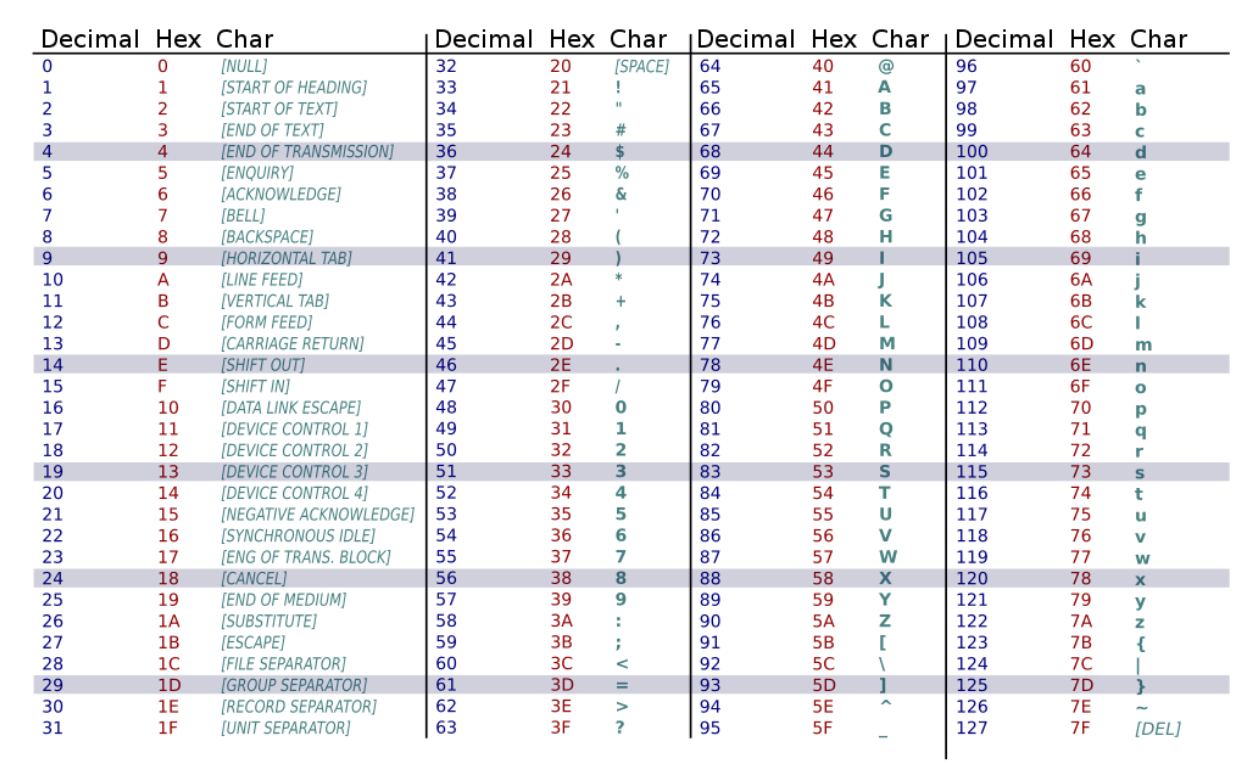
\includegraphics[width=\textwidth]{images/ascii_table.png}

\begin{multipart}
Let's say you are given a single character. If that character is a lowercase letter you must convert it to upper case. How can you do this without accidentally changing any other characters?
\end{multipart}

\vspace{1.5cm}

\begin{multipart}
How can you do this for every character of the string?
\end{multipart}

\vspace{1.5cm}

\begin{multipart}
Combine the previous two pieces into one piece of pseudocode:
\end{multipart}

\vspace{3cm}

\begin{multipart}
Consider what a sample run for your algorithm would look like. Where might something go wrong? Identify the ``boundary conditions" below:
\end{multipart}


\vspace{2cm}

\begin{multipart}
Write three sample inputs you can use to test your boundary conditions:
\end{multipart}
Sample 1:

\vspace{1.5cm}

Sample 2:

\vspace{1.5cm}

Sample 3:

\vspace{1.5cm}

\begin{multipart}
Implement your solution in C++ using VS Code. Revise your solution, save, compile and run it again. Are you getting the expected result and output? Keep revising until you do. Make you sure you test for the values used in your sample runs, and for the boundary conditions.
\end{multipart}

\subsection{Reading Tracker}
You are tasked with developing a reading tracker program that allows users to track their daily reading habits. Users can enter the genre of the book and the number of pages they read, and they can continue entering reading data until they decide to stop. The program should provide a summary of pages read by genre and calculate the total number of pages read for the day.


Your program should follow these guidelines:
\begin{enumerate}

 \item  Create 3 integer variables - Fiction, NonFiction, and Comics - to store the genre-wise totals.

 \item Allow the user to enter reading data by providing genre and pages. If they have already added pages to that genre, it should add the new value to the current total for that genre.

 \item Repeat this until the user decides to stop - which is done by inputting 'exit' in the genre prompt.

 \item If the user inputs a genre that doesn't exist, reprompt the user to input the right one.

 \item Display the genre-wise totals and calculate the total number of pages read for the day.
space is not visible).
\end{enumerate}
\begin{sample}
Enter a genre (Fiction, NonFiction, Comics, or 'exit'):

\textcolor{red}{Comics}

Enter the number of pages:

\textcolor{red}{30}

Enter a genre (Fiction, NonFiction, Comics, or 'exit'):

\textcolor{red}{NonFiction}

Enter the number of pages:

\textcolor{red}{40}

Enter a genre (Fiction, NonFiction, Comics, or 'exit'):

\textcolor{red}{Science}

Invalid Genre. Please enter a valid genre.
Enter a genre (Fiction, NonFiction, Comics, or 'exit'):

\textcolor{red}{Fiction}

Enter the number of pages:

\textcolor{red}{20}

Enter a genre (Fiction, NonFiction, Comics, or 'exit'):

\textcolor{red}{exit}

Genre-wise totals:

Fiction: 20 pages

NonFiction: 40 pages

Comics: 30 pages

Total pages read for the day: 90 pages

    
\end{sample}



\begin{multipart}
   Write out the steps you would use to solve this problem by hand as pseudocode.
\end{multipart}

\vspace{3cm}

\begin{multipart}
    Identify any boundary conditions for the problem.
\end{multipart}

\vspace{2cm}

\begin{multipart}
     Imagine how a sample run of your program would look like. Write at least two test cases:
\end{multipart}

Sample 1:

\vspace{1.5cm}

Sample 2:

\vspace{1.5cm}


\begin{multipart}
    Implement your solution in C++ using VS Code. Revise your solution, save, compile and run it again. Are you getting the expected result and output? Keep revising until you do. Make you sure you test for the values used in your sample runs, and for the boundary conditions.
\end{multipart}
\section{Homework}

\subsection{Print Collatz Sequence}

For this question, you will write a program that prompts the user to enter an integer value between 1 and 1000 (exclusive). Your program should then print out a sequence of numbers between the given value and 1 (inclusive) following the pattern below:
For a given number $a_i$,

\begin{itemize}
    \item If $a_i$ is even, then $a_{i+1} = floor(\frac{a_i}{2})$
    \item If $a_i$ is odd, then $a_{i+1} = 3a_i + 1$
\end{itemize}

Your program should stop printing numbers once the sequence reaches the value of 1.

If the user enters a number that is not between 1 and 1000 (exclusive), print ``Invalid input." and prompt the user for a number again.

This sequence is referred to as the Collatz sequence. The Collatz Conjecture states that this sequence will eventually reach the value of 1 for any starting number, a fact that has not yet been proven by modern mathematics!

Note: floor(x) means that x should be rounded down to the nearest integer.

\begin{sample}
    Enter a value between 1 and 1000:
    
\textcolor{red}{10}

10

5

16

8

4

2

1
\end{sample}

\begin{sample}
Enter a value between 1 and 1000:

\textcolor{red}{-5}

Invalid input.

Enter a value between 1 and 1000:

\textcolor{red}{17}

17

52

26

13

40

20

10

5

16

8

4

2

1
\end{sample}

\subsection{Potion Crafting}
You are creating a simple RPG video game, and you need to work out some details for your crafting menu. Your characters can craft two potions with simple ingredients: Minor Mana, and Minor Healing. The two potions have similar ingredients with some slight differences shown below.

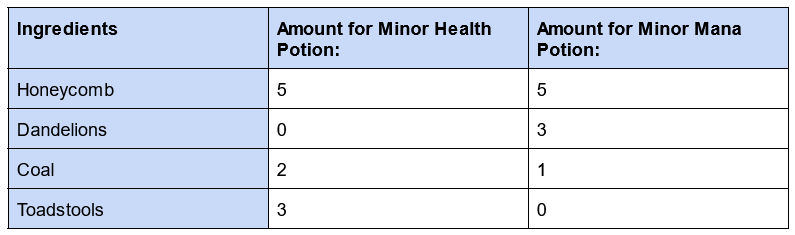
\includegraphics[width=\textwidth]{images/PotionIngredients.PNG}

You ask the user if they would like to prioritize Healing or Mana potions. It will then tell you how many you can produce of your priority potion, and then with the leftovers it will craft the other type of potion if it is possible. First ask for the priority potion, and then the quantities of the ingredients as an input. Then output how many of the priority potion you can make, and how many of the other potion. If the user provides an invalid input, ask them again.

\begin{sample}
Select a potion crafting priority:

1. Minor Mana

2. Minor Healing

\textcolor{red}{1}

How many Honeycombs do you have?

\textcolor{red}{14}

How many Dandelions do you have?

\textcolor{red}{8}

How many Coal do you have?

\textcolor{red}{4}

How many Toadstools do you have?

\textcolor{red}{6}

You can make 2 Mana potion(s) and 0 Healing potion(s).
\end{sample}

\begin{sample}
Select a potion crafting priority:

1. Minor Mana

2. Minor Healing

\textcolor{red}{4}

Invalid input. Select a potion crafting priority:

1. Minor Mana

2. Minor Healing

\textcolor{red}{2}

How many Honeycombs do you have?

\textcolor{red}{16}

How many Dandelions do you have?

\textcolor{red}{3}

How many Coal do you have?

\textcolor{red}{5}

How many Toadstools do you have?

\textcolor{red}{18}

You can make 2 Healing potion(s) and 1 Mana potion(s).
\end{sample}

\subsection{Most Popular Word}

A word is said to be most popular if it occurs more frequently than any other word. Write a function named MostPopularWord() that finds the most popular word in an array and print the most popular word, its frequency, and the indices where you found it. You may assume there's always one correct answer and the array will be non-empty. If it has equal occurrence, then we always consider the most recent one.

Note: You do not need sorting to solve this.

\textbf{Function:} Print the word with the highest frequency, its count, and its index positions in the array
\begin{quote}
\begin{itemize}
    \item \textbf{Name:} \mintinline{c++}{MostPopularWord()}
    \item \textbf{Parameters (Your function should accept these parameters IN THIS ORDER):}
        \begin{itemize}
            \item \mintinline{c++}{arr} String array: array of words.
            \item \mintinline{c++}{arrSize} int: The number of elements stored in the array
        \end{itemize}
    \item \textbf{Return Value:} void
\end{itemize}
\end{quote}


\begin{sample}

    \begin{minted}{c++}
    
    const int WORDS_SIZE = 4;
    string words[WORDS_SIZE] = {"mail", "text", "spam", "spam"};
\end{minted}
\textcolor{red}{Output:}

The most popular word : spam

Frequency : 2

Found at pos :

2

3
\end{sample}

\begin{sample}

    \begin{minted}{c++}
    
    const int WORDS_SIZE = 5;
    string words[WORDS_SIZE] = {"apple", "corn", "corn", "apple", "lettuce"};
\end{minted}
\textcolor{red}{Output:}

The most popular word : apple

Frequency : 2

Found at pos :

0

3
\end{sample}



\subsection{Weekly Expense Tracker}
Bob is trying to monitor his weekly expenses for better financial management. He is going through his logs and wants to find out the week he spent the least, the total amount spent, and the average weekly spending. To help Bob achieve this goal, write three functions: MinExpense(), TotalExpense(), and AverageExpense(). All three functions take two parameters: an array of doubles and the number of elements in the array. Then, they make the following computations:
\begin{itemize}
    \item \mintinline{c++}{MinExpense() } - returns the minimum value in the array
    \item \mintinline{c++}{TotalExpense()} - returns the sum of all the values in the array
    \item \mintinline{c++}{AverageExpense()} - returns the average of all the values in the array
\end{itemize}

You may assume that the array will be non-empty.

Function specifications:

\textbf{Function 1:} Finding the minimum hours studied
\begin{quote}
\begin{itemize}
    \item \textbf{Name:} \mintinline{c++}{MinExpense()}
    \item \textbf{Parameters (Your function should accept these parameters IN THIS ORDER):}
        \begin{itemize}
            \item \mintinline{c++}{arr} double array: The input array containing Bob's weekly expenses.
            \item \mintinline{c++}{arrSize} int: The number of elements stored in the array
        \end{itemize}
    \item \textbf{Return Value:} double: The minimum value in the array
\end{itemize}
\end{quote}


\textbf{Function 2:} Computing the total hours studied
\begin{quote}
\begin{itemize}
    \item \textbf{Name:} \mintinline{c++}{TotalExpense()}
    \item \textbf{Parameters (Your function should accept these parameters IN THIS ORDER):}
        \begin{itemize}
            \item \mintinline{c++}{arr} double array: The input array containing Bob's weekly expenses.
            \item \mintinline{c++}{arrSize} int: The number of elements stored in the array
        \end{itemize}
        
    \item \textbf{Return Value:} double: The sum of all the values in the array
\end{itemize}
\end{quote}


\textbf{Function 3:} Computing the mean study hours
\begin{quote}
\begin{itemize}
    \item \textbf{Name:}\mintinline{c++} {AverageExpense()}
    \item \textbf{Parameters (Your function should accept these parameters IN THIS ORDER):}
    \begin{itemize}
        \item \mintinline{c++}{arr} double array: The input array containing Bob's weekly expenses.
        \item \mintinline{c++}{arrSize} int: The number of elements stored in the array
    \end{itemize}
    \item \textbf{Return Value:} double: The average of all the values in the array

\end{itemize}
\end{quote}

\begin{example}
    Function call:

\begin{minted}{c++}
double arr[] = {1.24, 5.68, 3.456};
int arrSize = 3;
cout << "Min Expense: " << fixed << setprecision(2)<< MinExpense(arr, arrSize ) << endl;
cout << "Total Expense: " << fixed << setprecision(2) << TotalExpense(arr, arrSize ) << endl;
cout << "Average Expense: " << fixed << setprecision(2) << AverageExpense(arr, arrSize )
<< endl;
\end{minted}
    Output:

\begin{minted}{c++}
Min Expense: 1.24
Total Expense: 10.38
Average Expense: 3.46
\end{minted}
\end{example}

\begin{example}
    Function call:

\begin{minted}{c++}
double arr[] = {0};
int arrSize = 1;
cout << "Min Expense: " << fixed << setprecision(2)<< MinExpense(arr, arrSize ) << endl;
cout << "Total Expense: " << fixed << setprecision(2) << TotalExpense(arr, arrSize ) << endl;
cout << "Average Expense: " << fixed << setprecision(2) << AverageExpense(arr, arrSize ) << endl;
\end{minted}
    Output:

\begin{minted}{c++}
Min Expense: 0.00
Total Expense: 0.00
Average Expense: 0.00
\end{minted}
\end{example}

\subsection{Splitting a String}

When you're processing data, it’s useful to break up a text string into pieces using a delimiter. Write a function split() that takes a string, splits it at every occurrence of a delimiter, and then populates an array of strings with the split pieces, up to the provided maximum number of pieces.

Function specifications:

\begin{itemize}
    \item \textbf{Name:} split()
    \item \textbf{Parameters (Your function should accept these parameters IN THIS ORDER):}
    \begin{itemize}
        \item \mintinline{c++}{inputString} string: The text string containing data separated by a delimiter
        \item \mintinline{c++}{separator} char: The delimiter marking the location where the string should be split up
        \item \mintinline{c++}{arr} string array: The array that will be used to store the input text string's individual string pieces
        \item \mintinline{c++}{arrSize} int: The number of elements that can be stored in the array
    \end{itemize}
    \item \textbf{Return Value:} int: The number of pieces the input text string was split into
\end{itemize}

Note:
\begin{itemize}
    \item No input will have delimiters in the beginning or the end of the string. (Eg: ",apple, orange" OR "apple, orange,")
    \item No input will have multiple delimiters added consecutively. (Eg: "apple,,,orange,banana")
    \item If the delimiter character is not found, then the function returns 1 and the entire string is placed in the array as the first element.
    \item If the string is split into more pieces than the size of the array (the last parameter), then the function returns -1. The array should be filled with as many pieces of the split string as is possible.
    \item If an empty string is provided then return 0.
\end{itemize}

\begin{example}
Test code:
\begin{minted}{c++}
string testcase = "ABCDEFG";
char separator = ' ';
int arrSize = 3;
string arr[size];
// numSplits is the value returned by split
int numSplits = split(testcase, separator, arr, arr_size);
cout << "Function returned value: " << num_splits << endl;
cout << "arr[0]:"<< arr[0] << endl;
\end{minted}
Output:
\begin{minted}{c++}
Function returned value: 1
arr[0]: ABCDEFG
\end{minted}
\end{example}

\begin{example}
Test code:
\begin{minted}{c++}
string testcase = "RST,UVW,XYZ";
char separator = ',';
int arrSize = 3;
string arr[size];
// numSplits is the value returned by split
int numSplits = split(testcase, separator, arr, arrSize);
cout << "Function returned value: " << numSplits << endl;
for (int i=0; i < size; i++){
  cout << "arr["<< i << "]:" << arr[i] << endl;
}
\end{minted}
Output:
\begin{minted}{c++}
Function returned value: 3
arr[0]:RST
arr[1]:UVW
arr[2]:XYZ
\end{minted}
\end{example}

\begin{example}
Test code:
\begin{minted}[breaklines=true]{c++}
string testcase = "Bangkok,Berlin,Birmingham,Bogota,Busan,Baton Rouge,Beaumont,Boise,Budapest";
char separator = ',';
int arrSize = 5;
string arr[size];
// numSplits is the value returned by split
int numSplits = split(testcase, separator, arr, arrSize);
cout << "Function returned value: " << numSplits << endl;
for (int i=0; i < size; i++){
  cout << "arr["<< i << "]:" << arr[i] << endl;
}
\end{minted}
Output:
\begin{minted}{c++}
Function returned value: -1
arr[0]:Bangkok
arr[1]:Berlin
arr[2]:Birmingham
arr[3]:Bogota
arr[4]:Busan
\end{minted}
\end{example}
